\documentclass[12pt]{article}
\usepackage[margin=2.5cm]{geometry}
\usepackage[T1]{fontenc}
\usepackage{lmodern}
\input{glyphtounicode}
\pdfgentounicode=1
\usepackage{amsmath}
\usepackage{booktabs}
\usepackage{graphicx}
\usepackage{setspace}
\usepackage[running]{lineno}
\usepackage[numbers,super,sort&compress]{natbib}
\usepackage{url}
\usepackage{xr}
\externaldocument[S-]{supplement}
% params.tex: the numbers that the manuscript prints from results/, written by code/make_params.py;
% edit the script, never this file. Each number counts the population that its block names
% ("% Population:"), or the one that a [population: ...] note on its line names.
%
% Population tape: the dataset's tape records (신체정보데이터.zip), the subjects that carry every field the analysis reads
% Population images: the standing-pose label files of pillars A, B, D, F and H that carry the head, the torso and a foot, of the subjects in the tape population
% Population rig-images: the standing-pose label files of all 32 cameras that carry the head and a foot
% Population pose-images: the standing-pose label files of all 32 cameras
% Population hip-images: the standing-pose label files of pillar A that carry the head, a foot and the torso, of the tape subjects whose record gives the hip height
% Population subjects: the subjects with the widths in all six outfits, under the scale rule that the configuration names (the primary rule unless a macro's name says otherwise)
% Population none: a number that counts no population
% Crossing statureGainMin statureGainMax heelMedianCm heelShareMedian: the rise in the height in pixels, over pairs of photographs, against the recorded heel height over the tape subjects: the comparison that makes the primary scale rule and the no-heel rule bounds on the shoes' rise

% Design constants (code/reduction.py, code/read_560.py)
% Population: none
\newcommand{\nFolds}{5}
\newcommand{\nPartitionSeeds}{9}
\newcommand{\nBoot}{2{,}000}
\newcommand{\camerasTotal}{32}
\newcommand{\pillarsTotal}{8}
\newcommand{\camerasPerPillar}{4}
\newcommand{\ciLevel}{95}
\newcommand{\ciLowerPct}{2.5}
\newcommand{\ciUpperPct}{97.5}
\newcommand{\selfReportSdCm}{1}
\newcommand{\selfReportSdKg}{1.5}
\newcommand{\nDraws}{20}

% Counts (code/reduction.py)
% Population: subjects
\newcommand{\nTapeSubjects}{997}  % [population: tape]
\newcommand{\nSubjects}{706}
\newcommand{\nSuitSubjects}{750}  % [population: tape]
\newcommand{\nOwnSubjectsMin}{731}  % [population: tape]
\newcommand{\nOwnSubjectsMax}{747}  % [population: tape]

% Primary configuration: heel in own clothes only, the two widths (code/reduction.py)
% Population: subjects
\newcommand{\mapeBaseline}{3.31}
\newcommand{\rmseBaseline}{3.33}
\newcommand{\redSuit}{0.69}
\newcommand{\redOwnMin}{0.08}
\newcommand{\redOwnMax}{0.11}
\newcommand{\shortfallMin}{0.58}
\newcommand{\shortfallMax}{0.61}
\newcommand{\redSuitSeedMin}{0.67}
\newcommand{\redSuitSeedMax}{0.70}
\newcommand{\redOwnSeedMin}{0.06}
\newcommand{\redOwnSeedMax}{0.12}
\newcommand{\weightSuitDiffLo}{$-$0.36}
\newcommand{\weightSuitDiffHi}{0.17}
\newcommand{\weightOwnDiffLoMin}{1.42}
\newcommand{\growthIqrMin}{1.9}
\newcommand{\growthIqrMax}{2.2}

% Sensitivities: the other scale rules and the ellipse girth (code/reduction.py)
% Population: subjects
\newcommand{\nSubjectsNoHeel}{698}
\newcommand{\redOwnMaxAll}{0.12}

% Self-reported stature and weight: the main variant with the self-report error (code/reduction.py)
% Population: subjects
\newcommand{\selfBaseMin}{3.49}
\newcommand{\selfBaseMax}{3.74}
\newcommand{\selfRedSuitMin}{0.76}
\newcommand{\selfRedSuitMax}{0.98}
\newcommand{\selfRedOwnMin}{0.11}
\newcommand{\selfRedOwnMax}{0.24}

% The rig (code/rig.py)
% Population: rig-images
\newcommand{\legRatioDiagMin}{0.66}
\newcommand{\legRatioDiagMax}{0.74}
\newcommand{\legRatioSideMax}{0.11}
\newcommand{\legRatioRear}{0.98}
\newcommand{\statureGainMin}{1.2}
\newcommand{\statureGainMax}{1.3}
\newcommand{\heelMedianCm}{4.0}  % [population: tape]
\newcommand{\heelShareMedian}{2.4}  % [population: tape]
\newcommand{\nPhotographedSubjects}{981}  % [population: tape]
\newcommand{\torsoSideMax}{1.0}  % [population: pose-images]
\newcommand{\torsoOtherMin}{98.9}  % [population: pose-images]
\newcommand{\hipShareMin}{20}  % [population: hip-images]
\newcommand{\hipShareMax}{32}  % [population: hip-images]

% params_manual.tex -- the numbers that no result table or script in this repository derives: the versions of the
% software, and facts of the dataset's documentation that no script uses. Hand-edited; each line names its source.
% test_assertions.py reads this file beside params.tex.
% Population: none

% The software that ran the analysis (requirements.txt pins it; test_assertions.py compares the two).
\newcommand{\sklearnVersion}{1.8.0}     % requirements.txt: scikit-learn==1.8.0
\newcommand{\numpyVersion}{2.4.2}       % requirements.txt: numpy==2.4.2

% The dataset's documentation (the construction guide and the data manual that AI Hub distributes with it).
\newcommand{\buildYear}{2021}             % manual, meta table: 데이터 구축년도 2021년
\newcommand{\subjectsPlanned}{1{,}000}    % guide, 촬영 대상: 1,000 명의 한국 국적 남녀

% The article title, read by main.tex and by the separate title page so that the two cannot differ.
\newcommand{\papertitle}{In everyday clothing, waist widths of torso polygons hand-drawn on photographs add little to
the prediction of waist girth from stature, weight, sex and age}

\setcounter{secnumdepth}{0}

\title{\papertitle}
\date{}

\begin{document}
\maketitle
\doublespacing
\linenumbers

\begin{abstract}
Garment customization can obtain girths from photographs instead of a tape measure. Recent models predict girths from weight and the body's widths and depths in photographs of dressed people. A regression on
stature, weight, sex and age, which a customer can report without a photograph, also predicts girth, so the
photographs' contribution is the reduction in error relative to that regression. Whether clothing changes that contribution can be measured on a Korean dataset
whose adults were tape-measured and photographed in a close-fitting measurement suit and in five of their own outfits. We added two waist widths of torso polygons that labelers drew in the photographs, seen from the front and at $45^\circ$ to it, to a linear regression of the tape-measured waist girth
on stature, weight, sex and age, and scored both regressions on subjects not used to fit them. The widths lowered the mean absolute
percentage error by \redSuit\ percentage points in the suit but by \redOwnMin--\redOwnMax\ in each own outfit. The
suit's reduction exceeded each own outfit's under each assumption about shoe heels in converting pixels to centimeters,
and with an ellipse's girth in place of the widths. A regression on weight and the own outfits' two widths, which
stand in for the recent models' inputs with a diagonal width for the depth, predicted the girth less accurately than the regression without photographs.
Studies predicting waist girth from dressed photographs therefore need to report the error of the regression without
photographs on the same subjects.
\end{abstract}

\noindent\textbf{Keywords:} body measurement, waist girth, two-dimensional image, clothing, garment customization

\label{sec:intro}Mass customization of garments needs each customer's body dimensions. Measurement from
two-dimensional photographs obtains body dimensions remotely and without contact.\cite{zhang2025} A 2025 systematic
review of photograph-based body measurement named the restriction to a nude body or to tight-fitting clothing as a
limitation of the reviewed methods, and named estimation from the dressed body as a feasible approach for future
work.\cite{zhang2025}

Girths can be predicted from photographs of dressed people or without any photograph, from stature and weight. Feng et
al.\cite{feng2026} predicted young men's chest, waist and hip girths from photographs in which the men wore regular
shirts that were not overly loose. Their best models, linear regressions chosen among several sets of inputs and
algorithms, combined body weight with the body's width and depth in the photographs. Bartol et al.\cite{bartol2022}
predicted body measurements from stature and weight alone, by a linear regression that they fitted for each sex to a
dataset of three-dimensional body shapes reconstructed from body scans. On the body-shape dataset, the regression predicted
the waist girth with a lower mean absolute error than two methods that estimate the body shape from images. Bartol et al.\ proposed the regression as the baseline for later methods of body measurement.

Part of the accuracy that a model on dressed photographs reaches can therefore come from inputs that need no
photograph, such as weight. Every model that Feng et al.\ compared, across their sets of inputs and their algorithms,
used the widths and depths measured in the photographs, so the errors of those models do not show how much of the
accuracy the photographs supply. The photographs' contribution is the reduction in error, on the same subjects, when
widths measured in the photographs are added to a regression on stature, weight, sex and age. A customer can report all four inputs without a
photograph, because customers can estimate their own stature and weight.\cite{bartol2022} The photographs' contribution may also depend on clothing, the condition that restricts the reviewed methods.\cite{zhang2025} Measuring how clothing changes the
contribution requires subjects who were photographed both in minimal clothing and in everyday clothing and whose girths
were measured with a tape.

A Korean dataset that a government data portal distributes on application holds the photographs and the tape
measurements that measuring the effect of clothing requires.\cite{aihub560} The dataset holds tape measurements of
about \subjectsPlanned\ adults and photographs of the adults, taken from \pillarsTotal\ directions, in a close-fitting
measurement suit, which serves as minimal clothing, and in five outfits of the adults' own clothes. Labelers drew polygons around body parts in the photographs. The torso's polygon, on which widths can
be measured, rarely appears in photographs taken from the sides and mostly does not reach the hip, and the dataset gives
no height at which to locate the chest. We therefore added two waist widths, seen from the front and at $45^\circ$ to
the front, to a regression of the tape-measured waist girth on stature, weight, sex and age, and compared the reduction in error that the suit's widths bring with the reduction that
each own outfit's widths bring. The widths lowered the regression's mean absolute percentage error by \redSuit\
percentage points in the suit and by \redOwnMin--\redOwnMax\ percentage points in the own outfits. A regression on
weight and the own outfits' two widths, which takes the diagonal width in place of Feng et al.'s depth, predicted the
girth less accurately than the regression on stature, weight, sex and age.

\section{Materials and methods}\label{sec:methods}

\subsection{Data}\label{sec:data}

The dataset Whole Body Shape and Dimension Measurement Data for Koreans, built in \buildYear, holds photographs and body
dimensions of Korean adults.\cite{aihub560} AI Hub, a data portal of the Korean government, distributes the
dataset on application. The dataset's creators recruited about \subjectsPlanned\
adults, men and women in equal numbers. Trained measurers marked landmarks on each subject. They measured heights with
an anthropometer (a graduated vertical rod), girths with a tape measure and weight with a digital scale. The waist girth
is the horizontal circumference through the waist's side points, which lie at the natural indentation of the waist. The
measurers read the waist girth at mid-breath with the subject standing upright. The waist height, which locates the
waist in the photographs, is the vertical distance from the floor to a landmark that the measurers marked as the waist
point. Each subject's record also holds stature, weight, sex and age, and the heel height of the subject's shoes, which
raises the subject in photographs taken in shoes.

The creators photographed each subject in six outfits and six poses with \camerasTotal\ digital single-lens reflex
cameras, \camerasPerPillar\ at different heights on each of \pillarsTotal\ pillars around the subject. A
photograph's pillar sets the direction from which the photograph shows the waist. The creators supplied a measurement suit, which they chose
so as not to distort the body. The subjects brought the other five outfits from their own clothes: two for spring or
autumn, two for summer and one for winter without thick outerwear. Labelers drew polygons around body parts in each
photograph, including the head, the torso, the lower legs and the feet. We used the photographs of the standing
pose, in which the subject stands at attention. Of the \nTapeSubjects\ subjects whose records hold every value that the
analysis uses, \nPhotographedSubjects\ appear in the standing photographs.

\subsection{Camera positions and scale}\label{sec:rig}

Measuring the widths seen from the front and at $45^\circ$ needs each pillar's angle around the subject, but the
dataset does not record the pillars' angles. We inferred the angles from the lower legs in the measurement suit's
standing photographs (Figure~\ref{fig:rig}(a)). The dataset's file names number the cameras from 1 to
\camerasTotal, \camerasPerPillar\ to a pillar. We name the pillars A to H in the order of their camera numbers, so
pillar A holds cameras 1--\camerasPerPillar. Because a photograph's scale differs between cameras, we measure distances in units of the subject's
height in pixels, the vertical distance from the top of the head polygon to the lowest point of the foot polygons. The
leg offset, in these units, is the mean horizontal coordinate of the right lower-leg polygon's vertices minus the mean
horizontal coordinate of the left lower-leg polygon's vertices. For each camera, we took the median of the leg offset over
subjects. For each pillar, we averaged the cameras' medians over the pillar's cameras.

The leg offset is negative in pillar A, which means that the subject's right leg appears on the left of the image. The
subject therefore faces pillar A. A camera at the angle $\theta$ from the subject's front sees a horizontal distance
across the front shortened to $\cos\theta$ times its length. The ratio of a pillar's leg offset to pillar A's leg offset
is therefore about 0.71 at $\pm45^\circ$, 0 at $\pm90^\circ$, $-0.71$ at $\pm135^\circ$ and $-1$ at $180^\circ$. The
measured ratio is positive in pillars B and H and negative in pillars D, E and F (Figure~\ref{fig:rig}(a)). In absolute
value, the measured ratio is \legRatioDiagMin--\legRatioDiagMax\ in pillars B, D, F and H, \legRatioRear\ in pillar
E and at most \legRatioSideMax\ in pillars C and G. The ratios therefore place pillars B and H at $\pm45^\circ$ from the subject's
front, pillars D and F at $\pm135^\circ$, pillars C and G at $\pm90^\circ$ and pillar E at $180^\circ$. A line of sight
at $\pm135^\circ$ from the front lies at $45^\circ$ to the subject's front-back axis, as one at $\pm45^\circ$ does,
so the lines of sight of the four diagonal pillars B, D, F and H all lie at $45^\circ$ to that axis.

\begin{figure}[t]
\centering
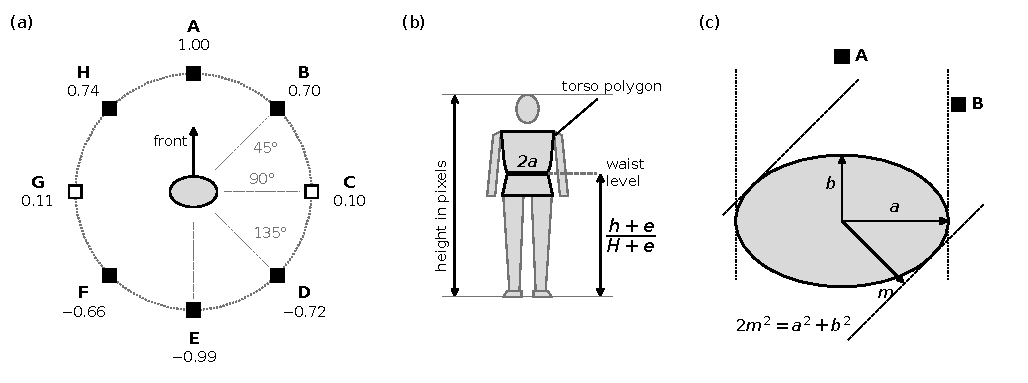
\includegraphics[width=\textwidth]{fig_rig}
\caption{The camera rig and the waist widths. (a) The \pillarsTotal\ pillars seen from above, with the subject's front toward
pillar A. The leg offset is the mean horizontal coordinate of the right lower-leg polygon's vertices minus the same mean for
the left lower-leg polygon, divided by the subject's height in pixels, the height from the head's top to the feet's lowest point.
The number under each pillar is the mean over the pillar's cameras of each camera's median leg offset in the
measurement suit, divided by the same mean for pillar A, and is negative where the legs appear in the opposite order to pillar A's photographs. Filled squares mark the pillars whose
photographs give the widths. The figure draws the pillars in the order of their camera numbers, because
the leg offsets fix each pillar's angle from the subject's front but not whether the pillar stands on the subject's left
or right side. (b) A front view, in which the waist level lies above the feet's lowest point by the fraction
$(h + e)/(H + e)$ of the height in pixels, where $h$ is the waist height, $H$ the stature and $e$ the heel height that
the scale rule adds for the outfit. The torso polygon's extent at that level is $2a$. (c) The waist section seen from above as an ellipse with semi-axes
$a$ and $b$. A camera sees the half-width between two tangents parallel to its line of sight: $a$ from pillar A, and $m$
from each diagonal pillar, such as pillar B. The two half-widths satisfy $2m^2 = a^2 + b^2$. Panels (b) and (c) are schematic.}
\label{fig:rig}
\end{figure}

To test whether the subjects wore shoes, we paired each own-outfit photograph of a subject with the same camera's
photograph of the subject in the measurement suit. For each pair, we divided the height in pixels in the outfit
by the height in pixels in the suit. For each own outfit, we took the median of this ratio over the pairs. The median exceeds 1 by
\statureGainMin--\statureGainMax\% in the five outfits, whereas the recorded heel height has a median of
\heelMedianCm~cm and a median of \heelShareMedian\% of stature over the subjects. We therefore take the subjects to have
stood barefoot in the measurement suit and in shoes in their own outfits, although the shoes raised the subjects less
than the recorded heel height. A length in centimeters is $S$ times the length in a photograph divided by the subject's
height in pixels, where $S$ is the subject's height in centimeters as photographed, shoes included. Three scale
rules, which differ in their assumptions about shoes, set $S$. Under the primary scale rule, which uses the only measure of
the shoes that the records give, $S$ is the measured stature in the suit and the stature plus the recorded heel height
in the subject's own outfits. Adding the heel height in every outfit shows whether a result depends on the subjects'
being barefoot in the suit. In the own outfits, adding no heel height gives a lower bound on the rise that the shoes
caused, and the primary rule gives an upper bound. A result that holds under all three scale rules therefore depends
neither on the subjects' being barefoot in the suit nor on how much the shoes raised them.

\subsection{Waist widths}\label{sec:features}

The labelers drew the torso in at most \torsoSideMax\% of pillar C's and pillar G's standing photographs and in at least
\torsoOtherMin\% of each other pillar's standing photographs, so the torso polygon gives widths but no depths. The
records also give the hip height, but the torso polygon spans the hip height's level in \hipShareMin--\hipShareMax\% of
pillar A's standing photographs per outfit. The records give no height for the bust points through which the chest
girth passes. The analysis therefore measures the torso polygon at the waist.

The two waist widths that the analysis adds to stature, weight, sex and age come from the standing photographs of
pillars A, B, D, F and H that show the torso and, for the height in pixels, the head and a foot. We took the frontal
half-width from pillar A alone and did not use pillar E, which sees the same extent from behind. Let $h$ be the
measured waist height, $H$ the measured stature and $e$ the heel height that the scale rule adds for the outfit. In each
photograph, the waist level lies above the lowest point of the feet by the fraction $(h + e)/(H + e)$ of the subject's
height in pixels (Figure~\ref{fig:rig}(b)). The half-width is the torso polygon's horizontal extent at the waist level,
divided by twice the height in pixels. For each of the \camerasPerPillar\ camera heights, $a$ is pillar A's half-width and $m$ the
mean of the half-widths that the diagonal pillars give.

A sensitivity analysis replaces the two widths with the girth of an ellipse fitted to the half-widths, to test whether
the photographs' contribution depends on the form in which the half-widths enter the regression. An ellipse with
the semi-axis $a$ from side to side and the semi-axis $b$ from front to back has the half-width
$\sqrt{a^2\cos^2\theta + b^2\sin^2\theta}$ seen at the angle $\theta$ from the front, so its half-width $m$ seen at
$45^\circ$ satisfies $2m^2 = a^2 + b^2$ (Figure~\ref{fig:rig}(c)). The waist section therefore matches such an ellipse only
when $2m^2 > a^2$. The ellipse's semi-axis $b$ is then $\sqrt{2m^2 - a^2}$. For each subject and outfit, we kept a camera height's half-widths when two conditions hold: pillar A and at least one
diagonal pillar give a half-width at that camera height, and $2m^2 > a^2$. The analysis with the widths and the
sensitivity analysis therefore use the same photographs and differ only in how the half-widths enter the regression.

The kept camera heights give each subject's widths and ellipse girth in each outfit. For each subject and outfit, the
frontal width is $2\bar{a}S$ and the diagonal width $2\bar{m}S$ in centimeters, where the bar denotes the mean over the
kept camera heights. A subject has widths in an outfit when at least one of the subject's camera heights in that outfit
is kept, which under the primary scale rule holds for \nSuitSubjects\ subjects in the measurement suit and for
\nOwnSubjectsMin--\nOwnSubjectsMax\ subjects in each own outfit. The subjects with widths in all six outfits enter the
models. The ellipse girth is $S$ times the mean, over the kept camera heights, of Ramanujan's approximation to the
perimeter of the ellipse with semi-axes $a$ and $b$,\cite{ramanujan1914}
\begin{equation}
\pi\bigl[3(a + b) - \sqrt{(3a + b)(a + 3b)}\bigr].
\end{equation}
The three scale rules and the two forms of the waist input, the widths or the ellipse girth, give six variants of the
analysis. The main variant uses the primary scale rule with the widths.

\subsection{Models and statistics}\label{sec:models}

The baseline model regresses the tape-measured waist girth on stature, weight, sex and age by ordinary least squares,
which scikit-learn (version \sklearnVersion) fits.\cite{pedregosa2011} For each outfit, the width model adds that
outfit's two widths to the baseline model's inputs. The weight-and-widths model regresses the girth on Feng et al.'s
inputs with the diagonal width in place of the depth, namely weight and the outfit's two widths.\cite{feng2026} All models are linear, as are the
best models of Feng et al.\ and the models of Bartol et al.,\cite{bartol2022} so that the comparisons concern the inputs and not the form of
the model. The subjects who enter the models depend on the scale rule, because the rule moves the waist level and so
changes which subjects have widths. \nSubjects\ subjects have widths in all six outfits under each scale rule that adds
a heel height, and \nSubjectsNoHeel\ subjects under the rule that adds none. Every model is fitted and scored on the
subjects who have widths in all six outfits under its scale rule.

To score every model on subjects that its fit did not use, we used scikit-learn's KFold to split the subjects at random
into \nFolds\ folds, groups of nearly equal size. Each fold's girths are predicted by a model fitted on the other folds.
Under each scale rule, every model uses the same split, so that a difference between two models does not depend on the
split.

The mean absolute percentage error (MAPE), the mean over subjects of $100|\hat{y} - y|/y$, where $y$ is the
tape-measured girth and $\hat{y}$ the prediction, measures each model's error. An outfit's reduction, the photographs'
contribution in that outfit, is the baseline model's MAPE minus the width model's MAPE for that outfit, in percentage
points (pp). A positive reduction means that the widths lower the error. For each own outfit, the shortfall, the part of
the photographs' contribution that the clothing removes, is the measurement suit's reduction minus that outfit's
reduction. The reduction in the root-mean-square error (RMSE), which gives the error in centimeters, is reported beside
the reduction in MAPE. Every difference is computed before rounding.

The confidence intervals come from bootstrap resamples, each of which draws subjects with replacement and recomputes
every MAPE and RMSE from the subjects' existing predictions, so every difference between two models compares their
errors on the same resampled subjects. The \ciLevel\% confidence interval of a difference in MAPE or in RMSE spans the \ciLowerPct{}th to \ciUpperPct{}th percentiles of
the difference over \nBoot\ such resamples,\cite{efron1993} which NumPy (version \numpyVersion) draws.\cite{harris2020}
The reductions are also recomputed under \nPartitionSeeds\ further random splits into folds, to measure how much the
reductions depend on the split. Because a customer reports stature and weight with error, a further analysis adds to both the self-report errors that
Bartol et al.\ assumed, normal with standard deviations of \selfReportSdCm~cm and
\selfReportSdKg~kg,\cite{bartol2022} and repeats the main variant's baseline and width models and its bootstrap for \nDraws\ random draws of the
errors.

\section{Results and discussion}\label{sec:results}

The baseline model predicts the tape-measured waist girth with an MAPE of \mapeBaseline\% and an RMSE of \rmseBaseline~cm
without any photograph. In the measurement suit, the widths lower the MAPE by \redSuit~pp, and in the subjects' own
clothes they lower it by \redOwnMin--\redOwnMax~pp (Table~\ref{tab:outfits}). The \ciLevel\% confidence interval of each own
outfit's reduction lies above zero. The shortfall is \shortfallMin--\shortfallMax~pp in the five outfits, so the
subjects' own clothes remove most of the suit's reduction. The \ciLevel\% confidence interval of each outfit's shortfall lies
above zero. Under the \nPartitionSeeds\ other fold splits, the suit's reduction ranges over
\redSuitSeedMin--\redSuitSeedMax~pp and the own outfits' reductions over \redOwnSeedMin--\redOwnSeedMax~pp.

The subjects' own clothes widen both waist widths in every outfit (Table~\ref{tab:outfits}). In every outfit and for
both widths, the interquartile range of the growth over subjects is \growthIqrMin--\growthIqrMax~cm, so the growth
differs between subjects. One reading of the shortfall is that a linear model's intercept and coefficients absorb the
part of the growth that all subjects share, whereas the part that differs between subjects adds to the error. Another
reading is that the labelers drew the torso's polygon less precisely in loose clothing than in the measurement suit.
The design does not separate one reading from the other.

In the five other variants of the analysis, the subjects' own clothes also remove most of the suit's reduction in
every own outfit (Supplementary Table~\ref{S-tab:sensitivity}). In the five other variants, the \ciLevel\% confidence
interval of every own outfit's shortfall also lies above zero. Whether the own outfits' reduction exceeds zero, however,
depends on the variant: the \ciLevel\% confidence interval of every own outfit's reduction includes zero under each scale
rule when the ellipse girth replaces the widths.

With the self-report errors added to stature and weight, the baseline model's MAPE rises from \mapeBaseline\% to
\selfBaseMin--\selfBaseMax\% over the \nDraws\ draws. In the same draws, the widths lower
the baseline model's MAPE by \selfRedSuitMin--\selfRedSuitMax~pp in the suit and by \selfRedOwnMin--\selfRedOwnMax~pp in the own outfits (Supplementary Table~\ref{S-tab:selfreport}).
In every draw, the \ciLevel\% confidence interval of each own outfit's shortfall lies above zero.

The weight-and-widths model is less accurate than the baseline model in the subjects' own clothes, whereas in the
measurement suit the data do not show which of the two models is more accurate (Table~\ref{tab:outfits}). In the
suit, the \ciLevel\% confidence interval of the weight-and-widths model's MAPE minus the baseline model's MAPE runs from
\weightSuitDiffLo\ to \weightSuitDiffHi~pp. In each own outfit, the lower bound of the same interval is
\weightOwnDiffLoMin~pp or above. A study that predicts the waist girth from dressed photographs needs to report,
beside its own error, the error that the regression on stature, weight, sex and age reaches on the same subjects,
because in the subjects' own clothes the widths add little to that regression and weight with the widths alone predicts
the girth less accurately than that regression.

The results have four limitations. First, the data come from one camera rig, one team of labelers and one population,
Korean adults. Second, the results concern the waist girth predicted without depths, so they do not test Feng et al.'s
models of the chest, waist and hip girths, which use depths. Third, labelers drew the polygons by hand, whereas a
customization service would extract the body's contour with software, which may trace loose clothing differently.
Fourth, the dataset names each own outfit only by its season and records no garment's ease, the allowance of a
garment's size over the body, so the growth of the widths cannot be traced to a property of the garments.

\begin{table}[t]
\centering
\caption{Waist girth prediction by outfit under the primary scale rule, for the \nSubjects\ subjects who have the
widths in all six outfits. The baseline model on stature, weight, sex and age has an MAPE of \mapeBaseline\% and an
RMSE of \rmseBaseline~cm. Width model: the MAPE of the model on the baseline model's inputs plus the outfit's frontal
and diagonal widths. Reduction: the baseline model's MAPE minus the width model's MAPE, with its \ciLevel\% bootstrap
confidence interval over subjects, and the same difference in RMSE with its interval. Shortfall: the measurement suit's reduction minus
the outfit's reduction. Weight + widths: the MAPE of the weight-and-widths model. Width growth: the median over subjects
of the outfit's width minus the suit's width. MAPE in \%, reductions and shortfalls in percentage points or in cm as
headed, widths in cm. Differences were computed before rounding.}
\label{tab:outfits}
\scriptsize
\setlength{\tabcolsep}{4pt}
\begin{tabular}{lrrlrlrlrrr}
\toprule
 & Width & \multicolumn{4}{c}{Reduction} & \multicolumn{2}{c}{Shortfall} & Weight + & \multicolumn{2}{c}{Width growth} \\
\cmidrule(lr){3-6}\cmidrule(lr){7-8}\cmidrule(lr){10-11}
Outfit & model & pp & \ciLevel\% interval & cm & \ciLevel\% interval & pp & \ciLevel\% interval & widths & Frontal & Diagonal \\
\midrule
Measurement suit & 2.62 & 0.69 & 0.53--0.85 & 0.60 & 0.39--0.79 & -- & -- & 3.21 & -- & -- \\
Spring/autumn 1 & 3.22 & 0.09 & 0.01--0.18 & 0.11 & 0.04--0.18 & 0.60 & 0.45--0.74 & 5.12 & 2.6 & 2.1 \\
Spring/autumn 2 & 3.21 & 0.11 & 0.03--0.19 & 0.10 & 0.04--0.16 & 0.58 & 0.43--0.73 & 5.16 & 2.7 & 2.2 \\
Summer 1 & 3.21 & 0.10 & 0.02--0.18 & 0.12 & 0.05--0.19 & 0.59 & 0.45--0.74 & 5.05 & 2.4 & 2.4 \\
Summer 2 & 3.23 & 0.08 & 0.01--0.15 & 0.09 & 0.03--0.14 & 0.61 & 0.46--0.75 & 5.04 & 2.4 & 2.3 \\
Winter & 3.23 & 0.08 & 0.02--0.14 & 0.06 & 0.00--0.12 & 0.61 & 0.45--0.76 & 5.28 & 2.8 & 2.2 \\
\bottomrule
\end{tabular}

\end{table}

\section{Conclusion}\label{sec:conclusion}

A regression on stature, weight, sex and age predicts girth without any photograph, so part of the accuracy that a model
on dressed photographs reaches can come from that regression's inputs alone. We measured what two waist widths in
photographs add to such a regression for Korean adults photographed in a measurement suit and in five of their own
outfits. The widths lowered the regression's mean absolute percentage error by \redSuit\
percentage points in the measurement suit, whereas in the subjects' own clothes they lowered the error by
\redOwnMin--\redOwnMax\ percentage points, by at most \redOwnMaxAll\ percentage points in any variant of the
analysis under any fold split, and by at most \selfRedOwnMax\ percentage points with the self-report errors added to
stature and weight. A regression on weight and the own outfits' widths alone predicted the waist girth less accurately than the
regression on stature, weight, sex and age.

\section*{Data availability}

AI Hub (\url{https://www.aihub.or.kr}) distributes the dataset Whole Body Shape and Dimension Measurement Data for
Koreans on application. The code that computes every number in this article from the dataset's polygons and tape records is
public.
The code's address is withheld from this anonymized version and given on the title page.

\bibliographystyle{vancouver-sage}
\bibliography{refs}

\end{document}
